\section{Issue 135: Uploading images from phone}

Issue 135 was to implement a feature allowing users to upload pictures from their phone/tablet to the the pictogram database. The feature was described as a userstory with the following description: "As a guardian, I would like a way to add pictograms by choosing an image from my phone gallery so that I can quickly improvise if the system does not have the activity I want." 
Initially we expected the feature to require a new screen and a new \gls{bloc} for handling communication with the api. We started out by designing the view, since the view should contain as little logic as possible the \gls{ui} should not have any influence on how the logic will be implemented. The \gls{ui} also served as a skeleton to implement and test the functionality while developing the final screen can be seen in \autoref{fig:uploadScreen}.

\begin{figure}[!h]
  \centering
  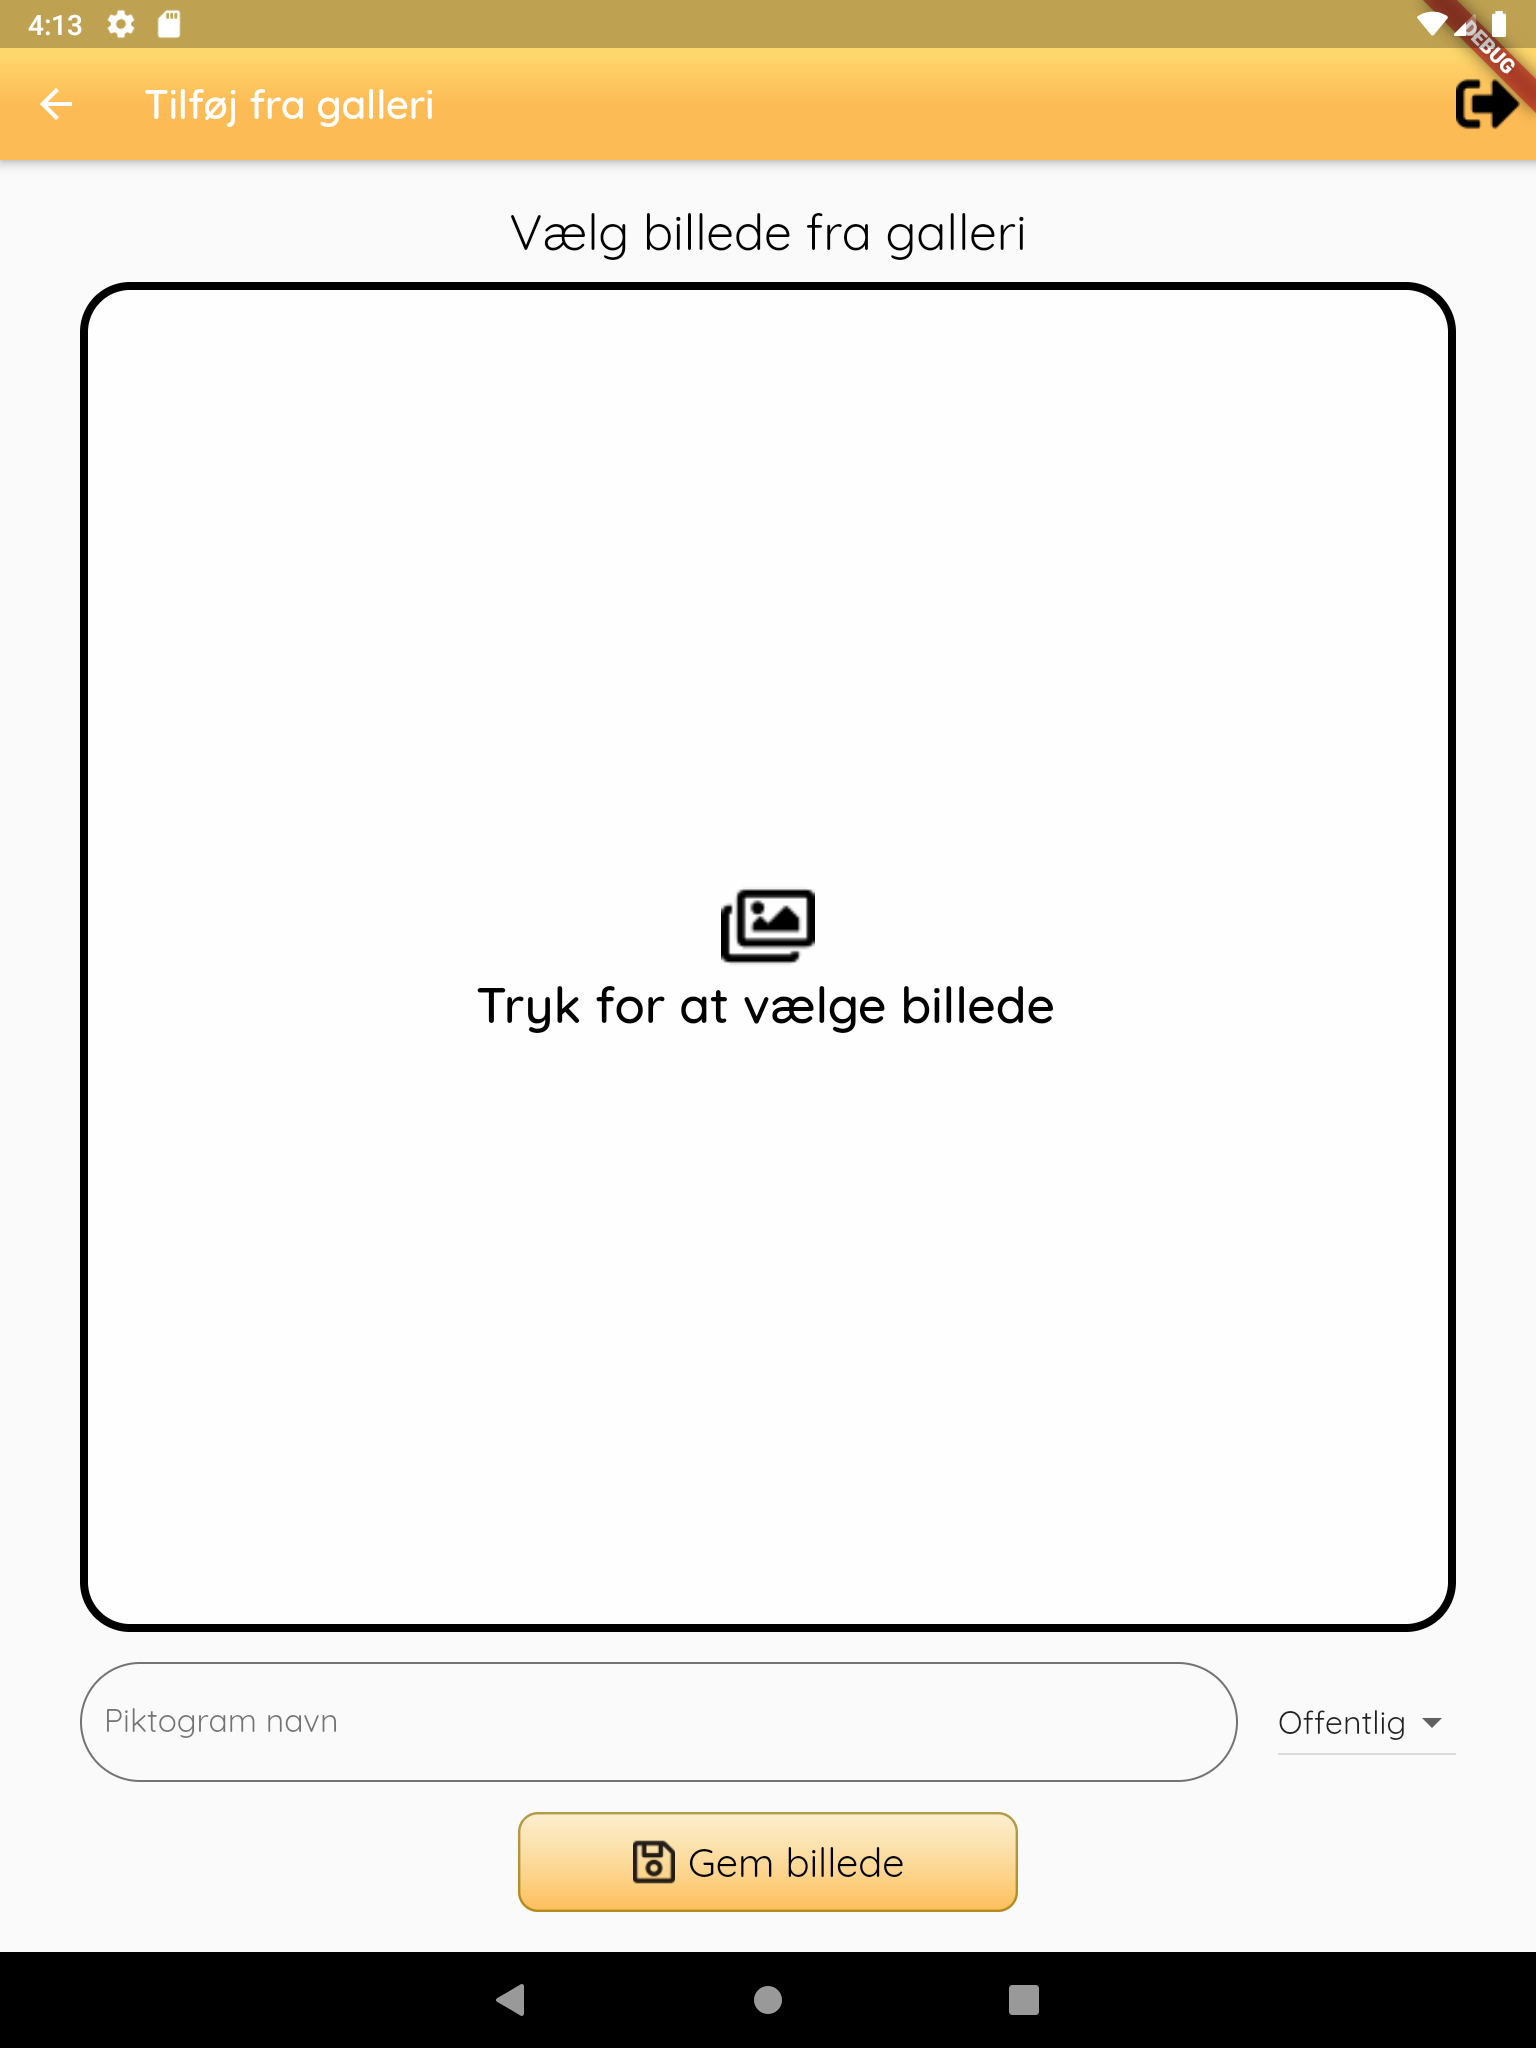
\includegraphics[width=0.7\textwidth]{figures/uploadPictogramScreen.png}
  \caption{Screenshot of the final implementation of the upload image screen}
  \label{fig:uploadScreen}
\end{figure}

For implementing the functionality of grabbing the image from the phone, a plugin was used, without any issues.
For uploading the image to the database we ran into many troubles, both in the \gls{fapi} where an endpoint was not fully implemented, bot also in the backend \gls{api} where there were some inconsistency between the specification and implementation of the endpoint we needed. the \gls{fapi} issue was caused no problems to implement, but the backend \gls{api} on had a flaw in the way it was coded, the endpoint for receiveing an image only accepting the image if it was in either png or in jpg format. But the logic for processing the image was made expecting the image to be in a byte array format. 
After changin this both api's were ready for sending and receiving images, but we also wanted to add som robustness for the picture uploading process, as currently if e.g the server crashed when receiving the image, it would leave a corrupt file. We added a layer of protection working when both creating a new image, or editing an existing one. The solution for creating a new image, was to mark an incoming image as temporary file, until it is done downloading, then if something went wrong the corrupt file will be easy to find and remove, as one can just remove images marked temporary. The same procedure was used for handeling updating/overwriting an existing image, here the incoming image is again marked as temporary, but the existing image is then marked as old, first when the incoming file is successfully download it the temporary mark will be removed and finally the old file will be deleted. This way the  the original image will not be lost if anything goes wrong during the download.

%%%%% INSERT IMAGE HER

This worked well when we hosted the backend locally and tested the functionality, but an intersting error ocurred when running it on the Giraf server. We ran into problems with implementation in dotnet core we found out that when we used the dotnet function \textit{System.IO.Move()} to remove the temporary tag from a new image by renaming it, this did not work when done in a Docker environment, due to a difference in how the filesystem handles links. This problem is that dotnet instead of renaming the file, it makes a hard-link with the new name instead, this works on filesystem on windows, but Docker does not handle this way, and hence the file was never renamed.